
\chapter{Klassendiagramme}
\section{Übersicht Klassendiagramm}

\begin{figure}[ht]
	\centering
	\includegraphics[width=\textwidth]{Klassendiagramm_Uebersicht}
	\caption{Klassendiagramm Übersicht}
\end{figure}

%\clearpage
%
%\section{Übersicht Methoden der Klassen}
%
%\begin{figure}[ht]
%	\centering
%	\subfigure[Klassendiagramm: ApplePayButton]{\includegraphics[width=0.49\textwidth]{KD_ApplePayButton}}
%	\subfigure[Klassendiagramm: CreditsPackage]{\includegraphics[width=0.49\textwidth]{KD_CreditsPackage}}
%	\caption{Klassendiagramme Teil 1}
%\end{figure}
%
%
%\begin{figure}[ht]
%	\centering
%	\subfigure[Klassendiagramm: CreditsPaymentProtocol]{\includegraphics[width=0.49\textwidth]{KD_CreditsPayment}}
%	\subfigure[Klassendiagramm: DatabaseProtocol]{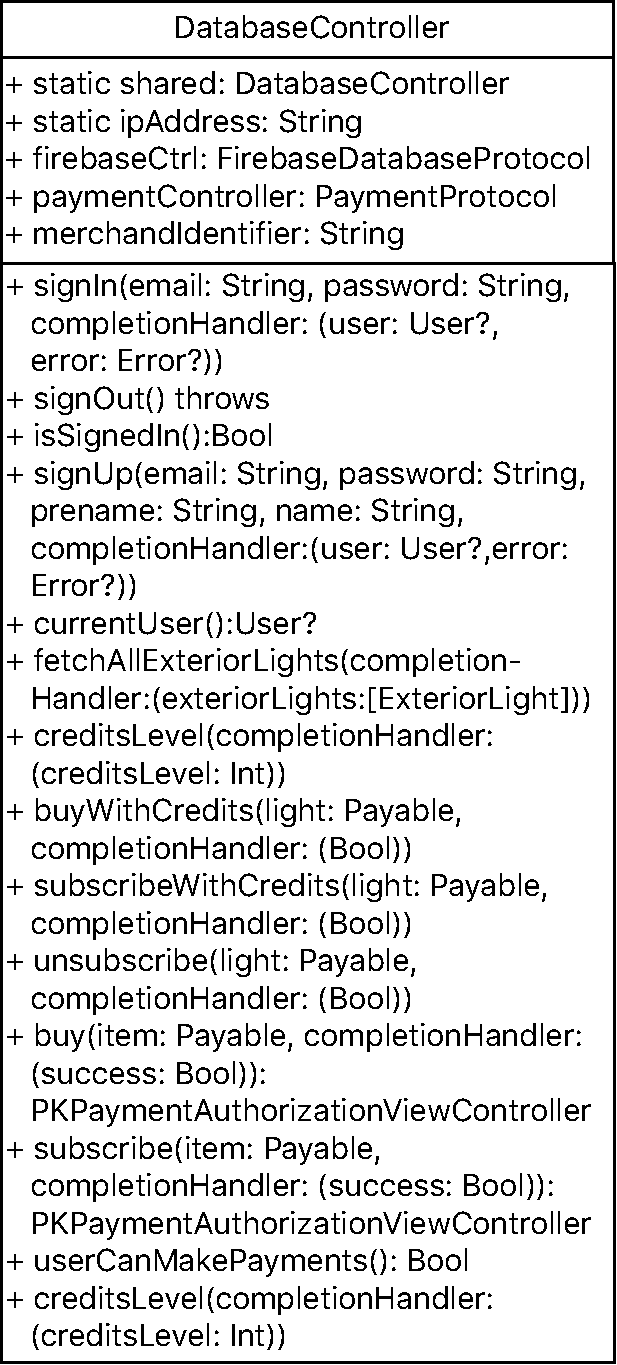
\includegraphics[width=0.49\textwidth]{KD_DatabaseController}}
%	\caption{Klassendiagramme Teil 2}
%\end{figure}
%
%
%\begin{figure}[ht]
%	\centering
%	\subfigure[Klassendiagramm: DecodeableProtocol]{\includegraphics[width=0.49\textwidth]{KD_DecodeableProtocol}}
%	\subfigure[Klassendiagramm: ExteriorLight]{\includegraphics[width=0.49\textwidth]{KD_ExteriorLight}}
%	\caption{Klassendiagramme Teil 3}
%\end{figure}
%
%
%\begin{figure}[ht]
%	\centering
%	\subfigure[Klassendiagramm: FirebaseDatabaseController]{\includegraphics[width=0.49\textwidth]{KD_FirebaseDatabaseController}}
%	\subfigure[Klassendiagramm: LightProtocol]{\includegraphics[width=0.49\textwidth]{KD_LightProtocol}}
%	\caption{Klassendiagramme Teil 4}
%\end{figure}
%
%\begin{figure}[ht]
%	\centering
%	\subfigure[Klassendiagramm: MoneyPaymentProtocol]{\includegraphics[width=0.49\textwidth]{KD_MoneyPaymentProtocol}}
%	\subfigure[Klassendiagramm: PackageProtocol]{\includegraphics[width=0.49\textwidth]{KD_PackageProtocol}}
%	\caption{Klassendiagramme Teil 5}
%\end{figure}
%
%\begin{figure}[ht]
%	\centering
%	\subfigure[Klassendiagramm: PaymentController]{\includegraphics[width=0.49\textwidth]{KD_PaymentController}}
%	\subfigure[Klassendiagramm: PaymentProtocol]{\includegraphics[width=0.49\textwidth]{KD_PaymentProtocol}}
%	\caption{Klassendiagramme Teil 6}
%\end{figure}
%
%\begin{figure}[ht]
%	\centering
%	\subfigure[Klassendiagramm: PKPaymentAuthorizationViewControllerDelegate]{\includegraphics[width=0.49\textwidth]{KD_PKPaymentAuthorizationViewControllerDelegate}}
%	\subfigure[Klassendiagramm: User]{\includegraphics[width=0.49\textwidth]{KD_User}}
%	\caption{Klassendiagramme Teil 7}
%\end{figure}

